\chapter{高級言語と低級言語の計算時間には差があるか}
\vspace{-1cm}
\section{実験の目的}
Java言語とアセンブリ言語で,計算時間に差があるかを明らかにする.

\section{実験方法}
Javaのソースコードの2行目を\\
\verb+int[] data = new int [データ数]+\\
とし,実験を行う.実行コマンドは以下である.
\begin{lstlisting}[numbers={none},caption={Javaコンパイル,実行時間の計測}]
$ javac sort.java
$ java sort
\end{lstlisting}
また,アセンブリで記述したプログラムの計測は\ref{fig:アセンブリ計測}を参照.

\section{実験結果}
\begin{figure}[htbp]
  \centering
  \begin{minipage}{0.45\textwidth}
    実験の結果,右の表が得られた.
  \end{minipage}
  \begin{minipage}{0.45\textwidth}
    \caption{実行時間の比較}
    \label{fig:実行時間の比較}
    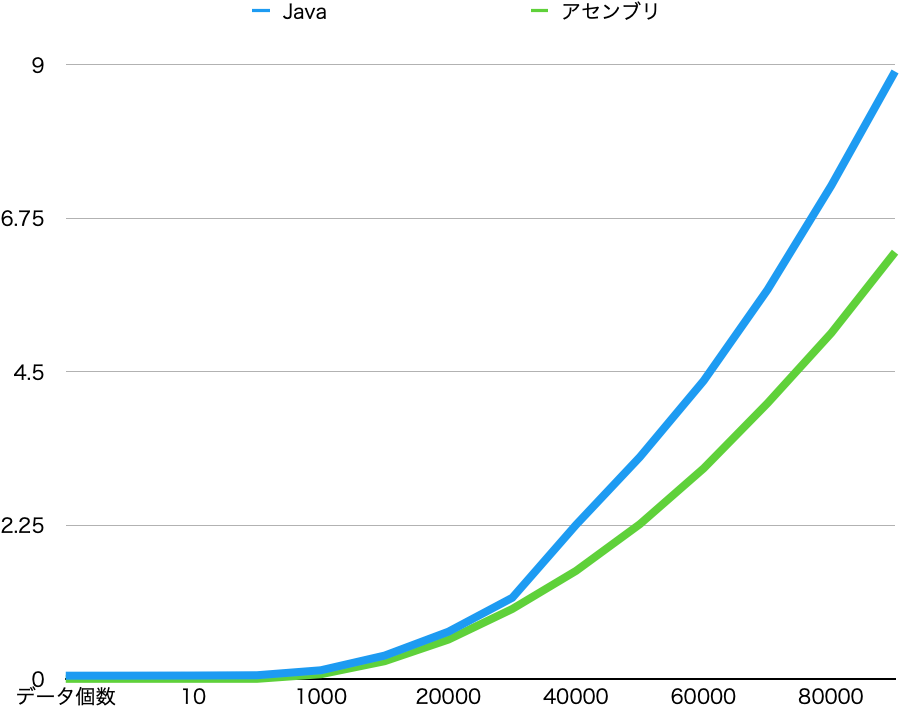
\includegraphics[scale=0.45]{Sec4.png}
    \end{minipage}
\end{figure}

\section{考察}
実験結果から,選択ソートアルゴリズムに関しては高級言語よりも低級言語のほうが,データ数によっては実行時間が早くなることが明らかとなった.同じ処理なのに実行時間に差が出る理由は,今回使用した高級言語であるJava言語が命令を一つづつ機械語に翻訳していくインタプリタ方式を採用していることに由来していると考えられる.
